%!TEX root = Report.tex
\chapter{Measurements And Results}\label{sec:results}

\section{Flow Field}

For better results, we are only comparing the last two (second and third run), because the flow and heat distribution is developed and steady.  As the results obtained by both runs are qualitatively similar in respect to the flow characteristics, only the second run is going to be taken as representative for the interpretation of our flow. In the second section of this chapter, a comparison between both runs is going to be made.

\begin{figure}[H]
\centering
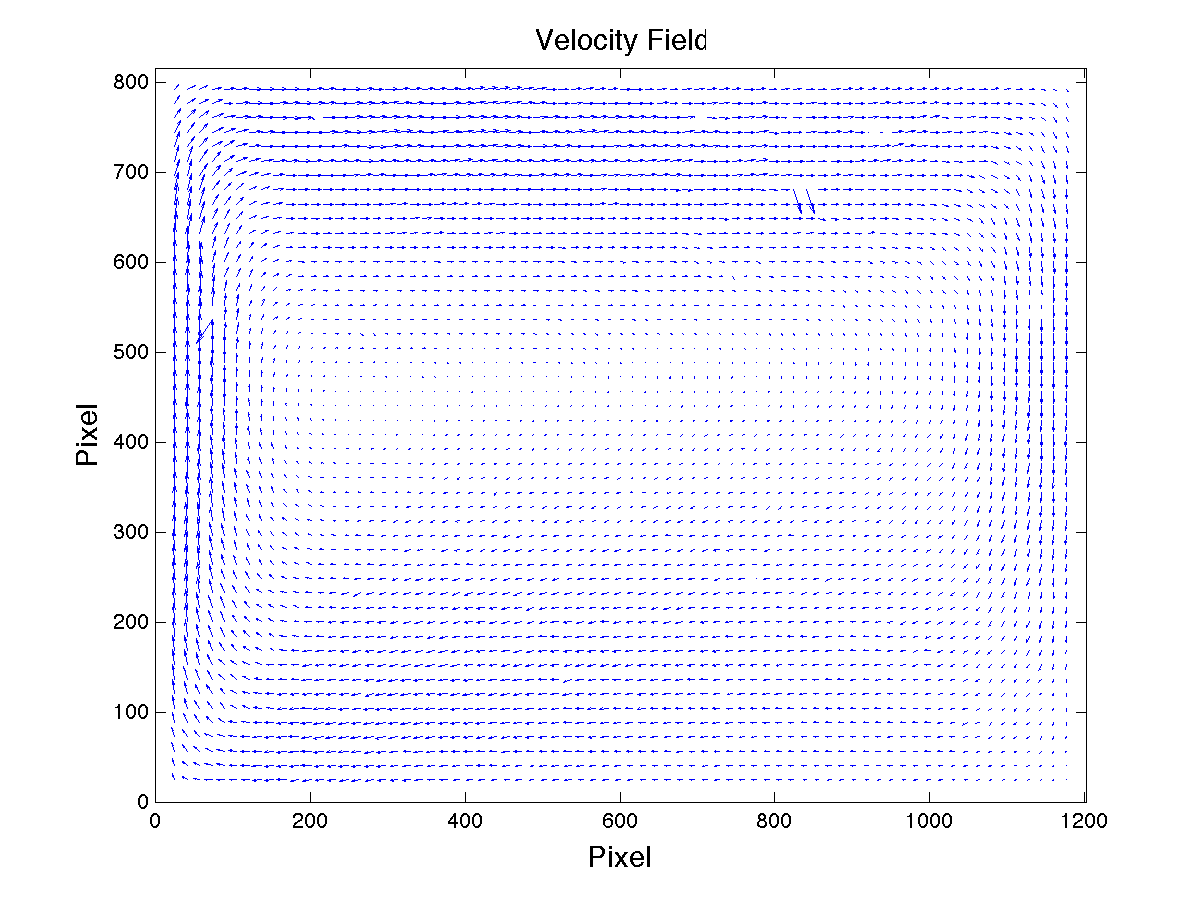
\includegraphics[width=0.65\textwidth]{pics/figure2_run2.png}
\caption{Flow Field For The Second Run}
\label{pic:2r2}
\end{figure}

We see in Figure \ref{pic:2r2} the calculated Flow field of our experiment. We don't see a significant difference between the flow fields. As expected, we obtained a circular flow generated by the heat convection at the heating wall. Because we're dealing with a fluid, the continuity equation tells us that the flow lines have to be closed (Figure \ref{pic:3r2}) and therefore at the right (and colder) part of the probe, the flow goes towards the bottom. \\


\begin{figure}[H]
\centering
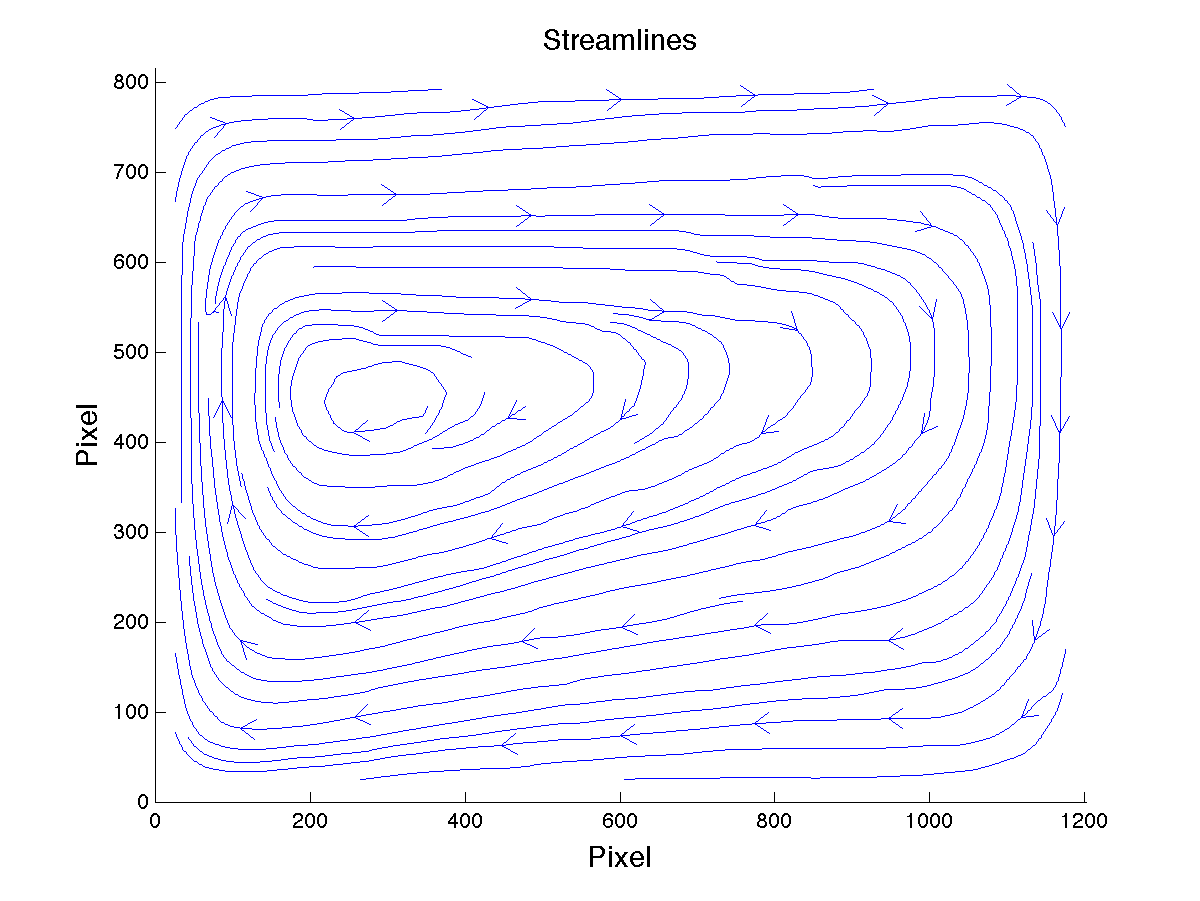
\includegraphics[width=0.65\textwidth]{pics/figure3_run2.png}
\caption{Field Lines For The Second Run }
\label{pic:3r2}
\end{figure}

As mentioned, the continuity equation ($\nabla \cdot \vec  v$ = 0, where $\vec v$ is the flow field) tells us that the divergence of the flow field is expected to be zero. In Figure \ref{pic:4r2} we see that the divergence behaves very homogeneously throughout the measured field and always shows values close to 0. 

\begin{figure}[H]
\centering
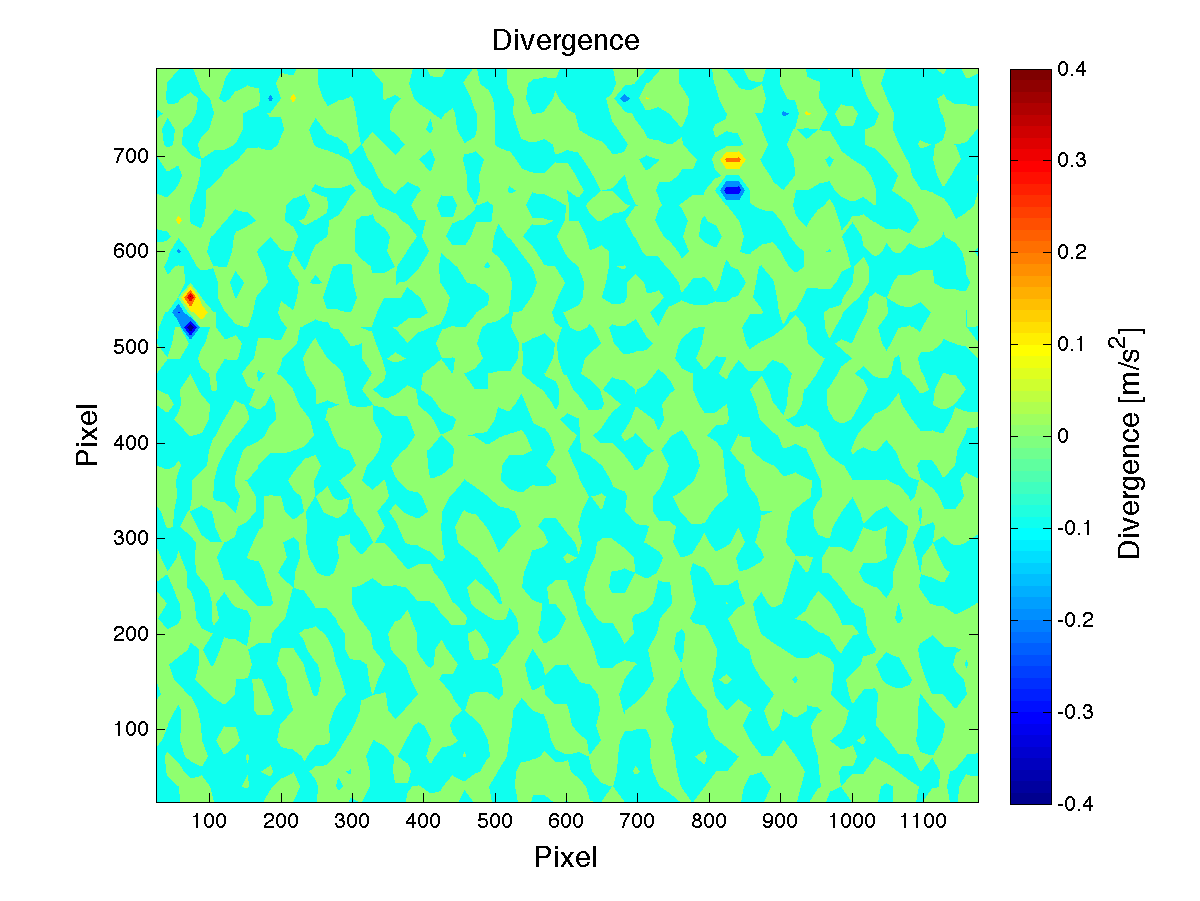
\includegraphics[width=0.65\textwidth]{pics/figure4_run2.png}
\caption{Divergence For The Second Run}
\label{pic:4r2}
\end{figure}

This is a good indicator for the quality of our results. In some spots tough, the divergence field shows a inhomogeneous behaviour (significantly higher deviation to zero), but the corresponding flow flield manifestates also with a clear erratic behaviour (very small flow vector or illogical flow direction compared to the sorrounding flow field) which is not taken in consideration anyway. The source of these errors is probably caused by the correlation formula that has has difficulties finding the patern in of the interrogation area.\\

We see from the previous figures, that the stream lines have the strongest curvature towards the center of the analysed area, so the curl is expected to be also higher towards the center, which is confirmed by Figure \ref{pic:5r2}, that show the curl of the flow field. Here, again, we spot some small areas with erratic behaviour. This is again direct consequence of the irregular flow velocities calculated above.




\begin{figure}[H]
\centering
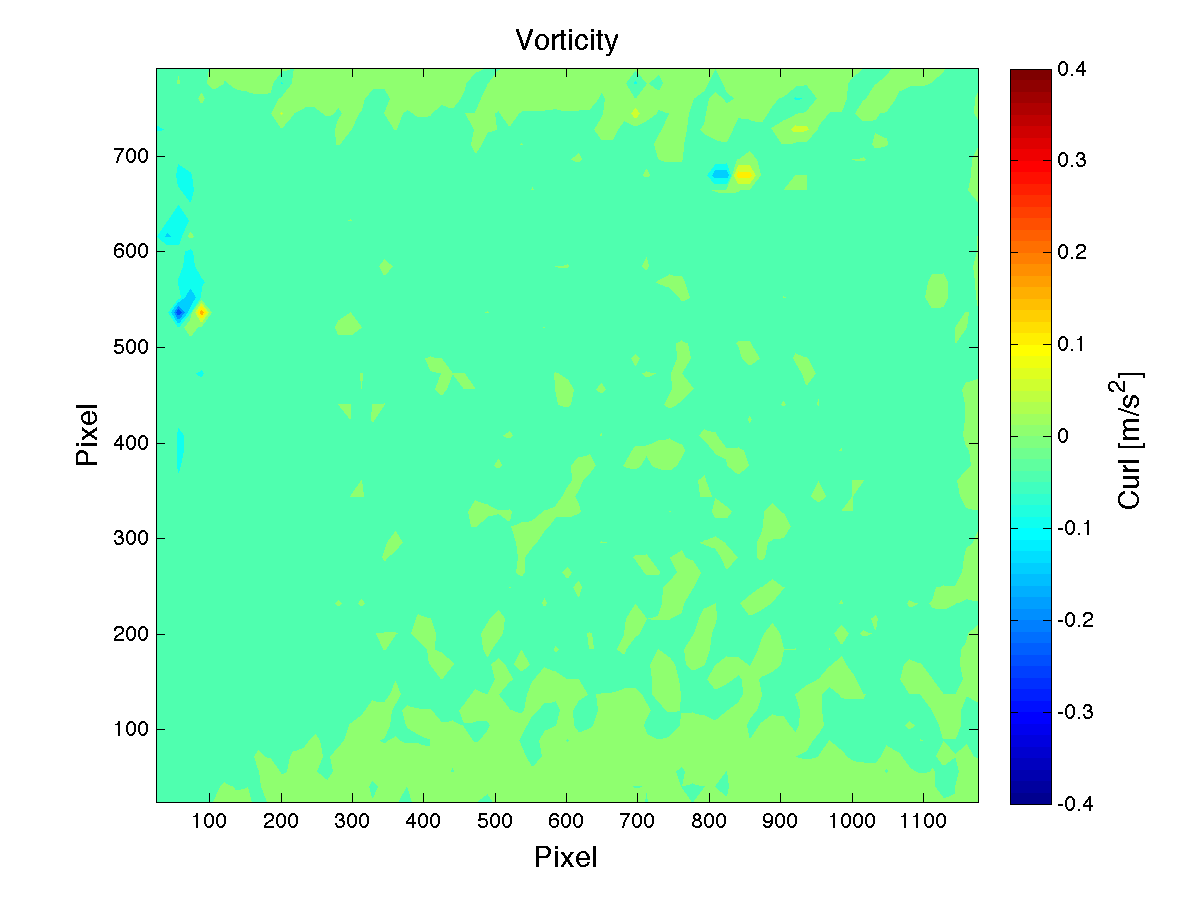
\includegraphics[width=0.65\textwidth]{pics/figure5_run2.png}
\caption{Curl For The Second Run}
\label{pic:5r2}
\end{figure}






\section{Influence Of Aperture Setting}

In this section, the results for the third run are going to be compared with the showed ones corresponding the second one. As it was mentioned previously in the resport, the exposure time at the third run was higher than at the second. To keep the amount of light constant the shutter aperture was decreased. The optical effect of the latter makes the focusing depth bigger, on the other hand the higher exposure makes the position of the particle more blurred as they move during the time the photograph is being taken.\\



\begin{figure}[H]
\centering
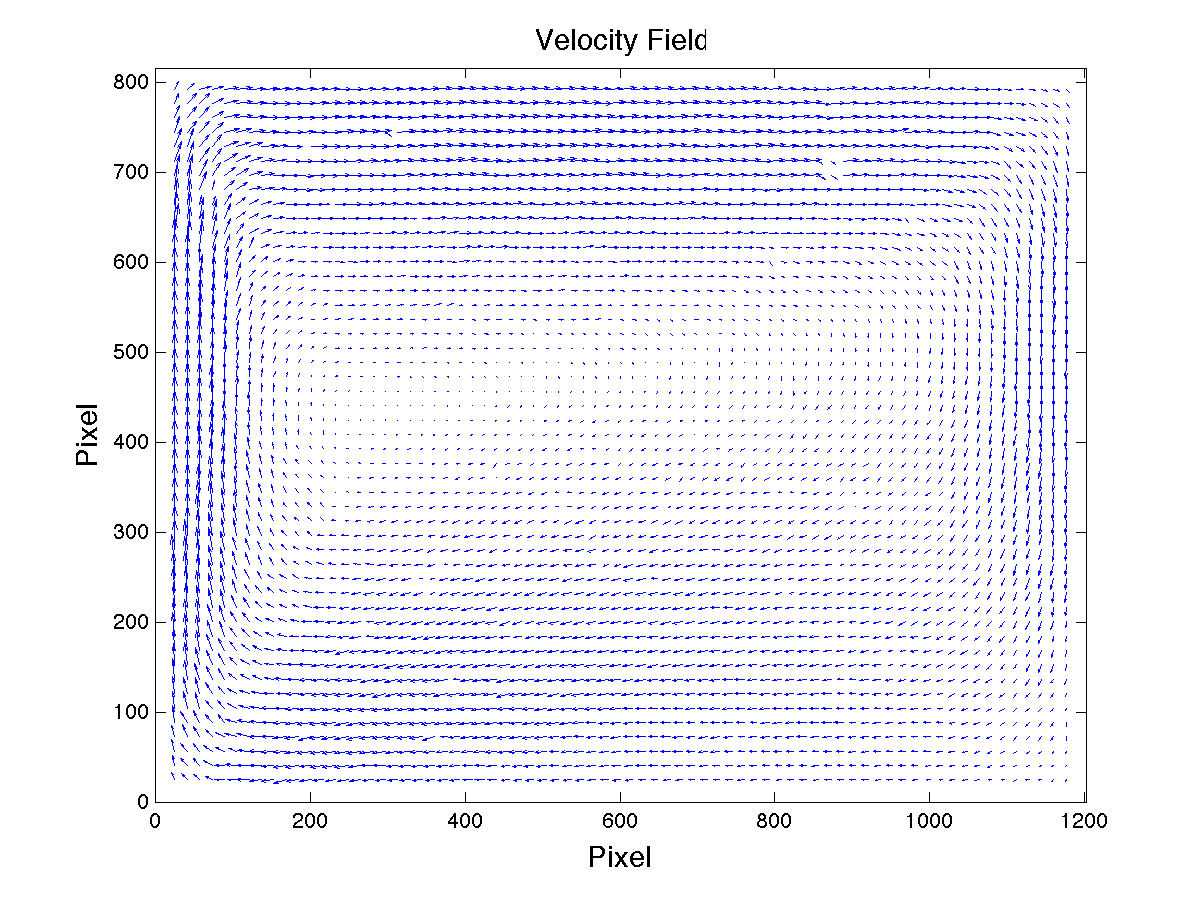
\includegraphics[width=0.65\textwidth]{pics/figure2_run3.png}
\caption{Flow Field For The Third Run}
\label{pic:2r3}
\end{figure}

The higher exposure and the produced blurriness gives the constelations more "individuality" so that they are harder to get confused as other constelations by our correlation function. This is the reason why the results in the third run are slightly better than the ones in the second run. In the Appendix (Figures \ref{pic:1r2} and \ref{pic:1r3}) we see also how the correlation of the third run is in general a little better (smaller, clearer points) than the one of the second.


\begin{figure}[H]
\centering
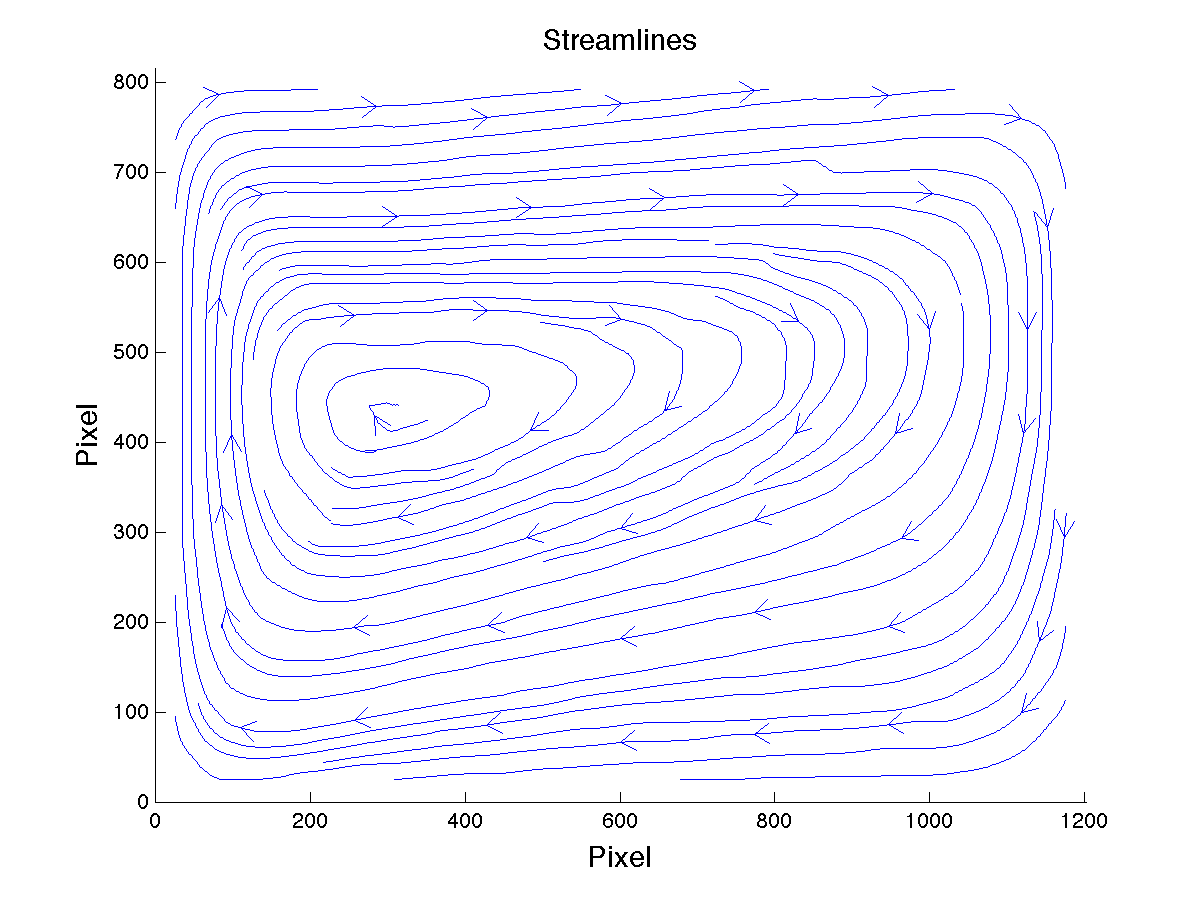
\includegraphics[width=0.65\textwidth]{pics/figure3_run3.png}
\caption{Field Lines For The Third Run}
\label{pic:3r3}
\end{figure}

What we could observe in the flow  (Figure \ref{pic:2r3}) is a more even velocity field, i.e. the amount of discrepancies and erratic behaviour was decreased. Qualitatively, the flow field looks very similar to the previous one altough the exposure time was increased by more than $80\%$. 


\begin{figure}[H]
\centering
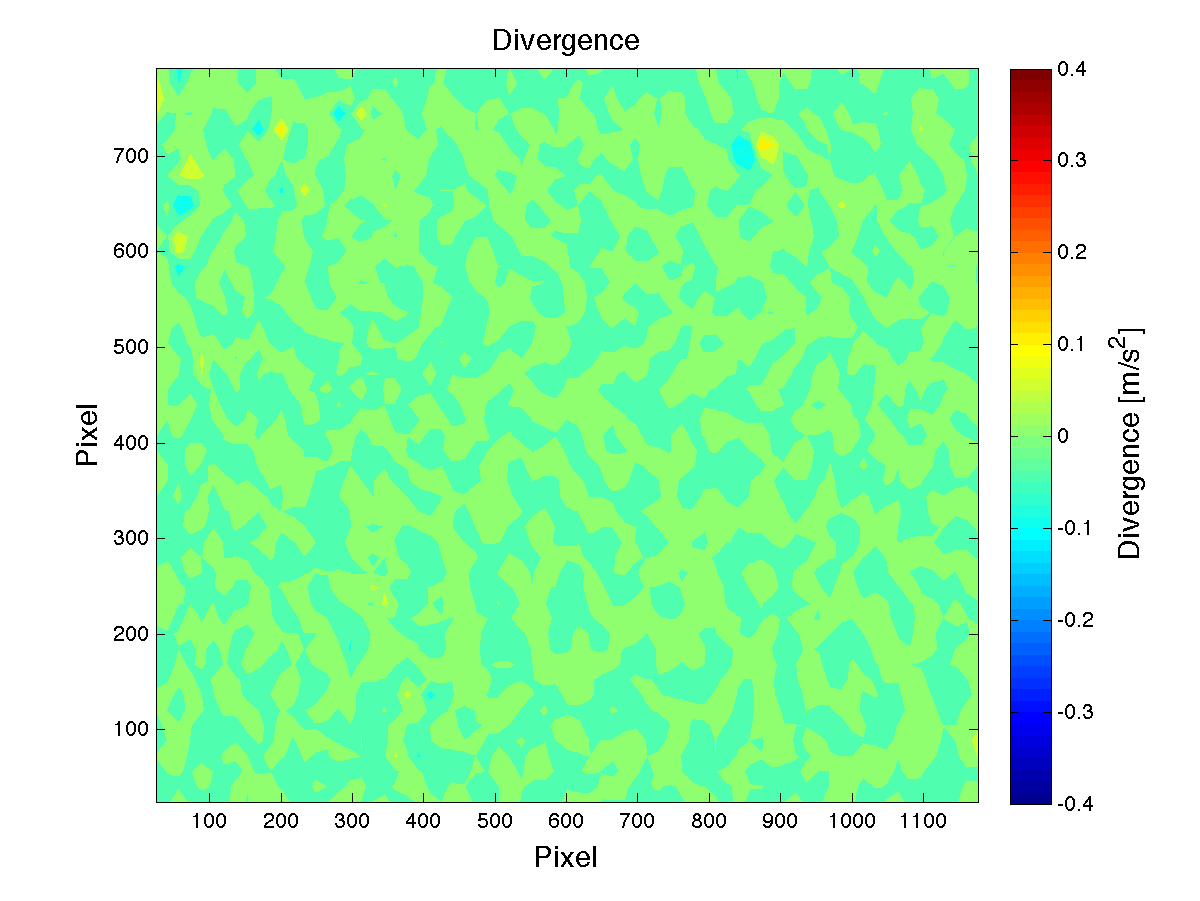
\includegraphics[width=0.65\textwidth]{pics/figure4_run3.png}
\caption{Divergence For The Third Run}
\label{pic:4r3}
\end{figure}

For the mentioned reasons, the streamlines calculated seem to develop smoother (Figure \ref{pic:3r3}) and the divergence oscilates more harmoniously around zero, as expected (Figure \ref{pic:4r3}). We can still spot some numerical irregularities in the divergence and curl field, but they have much lower peaks than in the second run.


\begin{figure}[H]
\centering
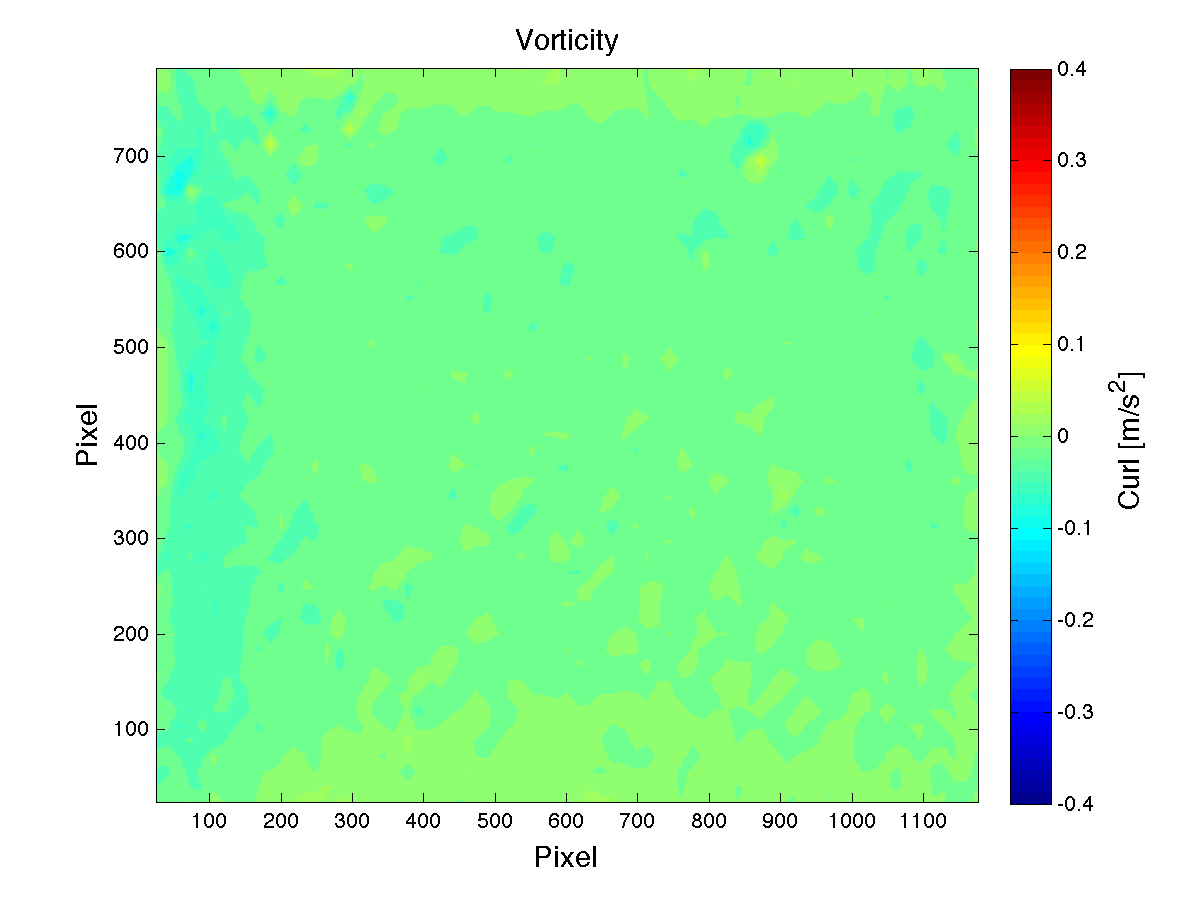
\includegraphics[width=0.65\textwidth]{pics/figure5_run3.png}
\caption{Curl For The Third Run}
\label{pic:5r3}
\end{figure}

If we observe Figure \ref{pic:compared} we observe that the different exposure times and shutter appertures used (Table \ref{tab:exposure}) don't really make any notable difference on the pictures taken for our experiments. The results obtained and showed above behave rather plausible tough. For a better comparison in the effects of the different optic setup one should analyse the results for more extreme differences in the exposure time and shutter apperture. 

\begin{figure}[H]
\centering
\mbox{
\subfigure[]{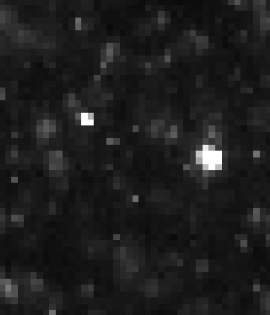
\includegraphics[width=.37\textwidth]{pics/croprun2.png}
\label{pic:crop2}}\quad
\subfigure[]{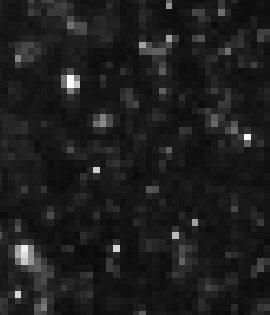
\includegraphics[width=.37\textwidth]{pics/croprun3.png}
\label{pic:crop3}}}
\caption{Extraction of Image in Run 2 (left) and Run 3 (right)}
\label{pic:compared}
\end{figure}

One of the main problems of the PIV method is the Peak Locking effect, where the velocities (or displacements) show an inhomogeneous behaviour on the grid. In Figure \ref{pic:6r2} we put all the displacements of the second run together that are exactly on an integer pixel value and those that have a value inbetween. We see clearly a peak locking effect or an effect of displacements being "rounded" to the next complete pixel value. Because the displacements histogram for the third run look very similar to the one showed above, the one for the third run is shown in the Appendix (Figure \ref{pic:6r3}). 

\begin{figure}[H]
\centering
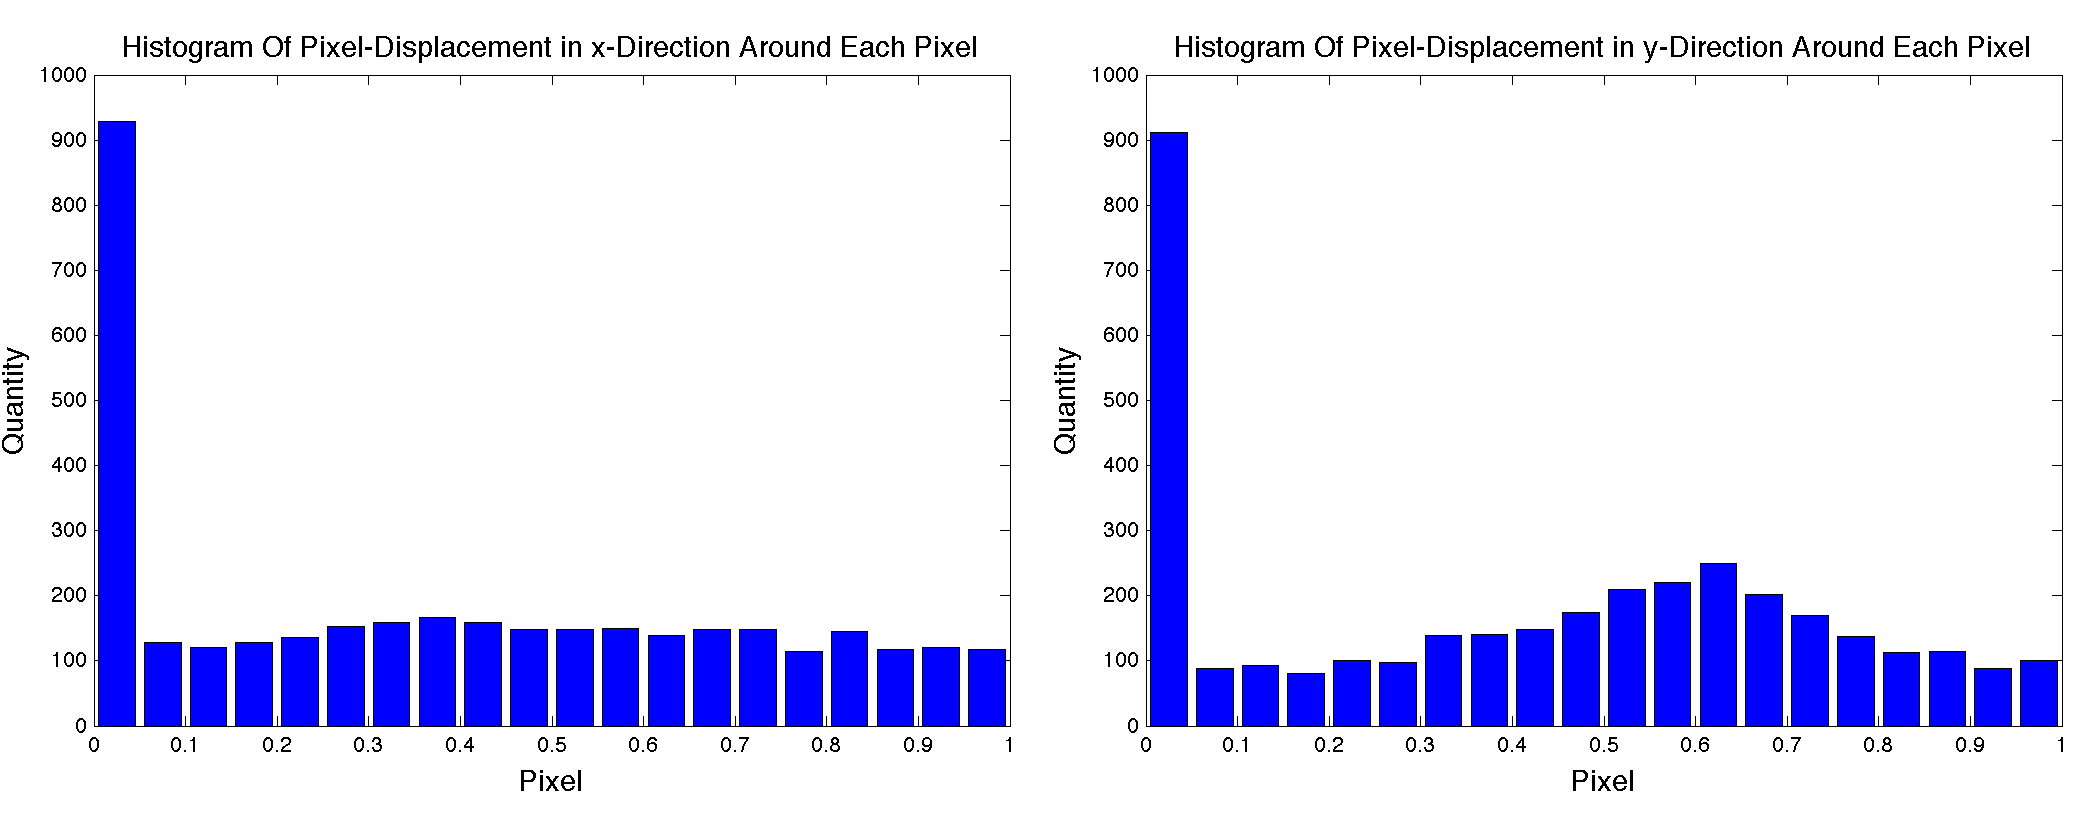
\includegraphics[width=0.9\textwidth]{pics/figure6_run2.png}
\caption{Histograms Of Displacements in $x$ and $y$ Directions For The Second Run}
\label{pic:6r2}
\end{figure}